\section{Kodowanie korekcyjne Reeda-Solomona}
\subsection{Wstęp}

Kodowanie korekcyjne Reeda-Solomona zostało stworzone przez Irvina S. Reeda
oraz Gustava Solomona w 1960 roku~\cite{Reed-Solomon-original}

Kody Reeda-Solomona charakteryzują się kilkoma parametrami~\cite{Reed-Solomon-Encoding-Decoding}:
\begin{itemize}
    \item alfabetem w ciele skończonym $\mathbb{F}_{p^m}$, $m>1$, $p$ jest liczbą
    pierwszą
    \item długością wiadomości $k$ do zakodowania $k < 2^{m}$
    \item długością słowa kodowego $n$ gdzie $k < n < 2^{m}$
    \item wielomianem generującym $g(x)$ dla kodów BCH
\end{itemize}

W kodach Reeda-Solomona wykorzystywanych w Ethernecie wykorzystujemy ciało $\mathbb{F}_2$ oraz ciała rozszerzone
$\mathbb{F}_{2^m}, m \in \{ 2, 3, \ldots \}$.

\subsection{Ciało skończone $\mathbb{F}_{q}$}

Aby zrozumieć działanie kodu Reeda-Solomona, trzeba najpierw zrozumieć, czym jest
ciało skończone $\mathbb{F}_q$ zwane też ciałem Galois $\operatorname{GF}(q)$.
Ciało to jest ciałem $K$ rzędu $q$, czyli takie, które zawiera jedynie $q$ elementów.
Aby struktura algebraiczna była ciałem, musi definiować 2 operacje zwane
dodawaniem i mnożeniem.
Te operacje muszą spełniać kilka warunków:

{\small
    \begin{align}
        a + (b + c) &= (a + b) + c & \forall a,b,c &\in K && \text{Łączność dodawania} \\
        a \cdot (b \cdot c) &= (a \cdot b) \cdot c & \forall a,b,c &\in K && \text{Łączność mnożenia} \\
        a + b &= b + a & \forall a,b &\in K && \text{Przemienność dodawania} \\
        a \cdot b &= b \cdot a & \forall a,b &\in K && \text{Przemienność mnożenia} \\
        a + 0 &= a & \forall a &\in K && \text{Element neutralny (0) dodawania} \\
        a \cdot 1 &= a & \forall a &\in K && \text{Element neutralny (1) mnożenia} \\
        a + (-a) &= 0 & \forall a &\in K && \text{Element odwrotny (-a) dodawania} \\
        a \cdot a^{-1} &= 1 & \forall a &\in K \setminus \{ 0 \} &&
            \text{Element odwrotny (} a^{-1} \text{) mnożenia} \label{field_mul_inverse}\\
        a \cdot (b + c) &= (a \cdot b) + (a \cdot c) & \forall a,b,c &\in K &&
            \text{Rozdzielność mnożenia względem dodawania}
    \end{align}
}%

Aby stworzyć ciało rzędu $p$ gdzie $p$ jest liczbą pierwszą, można wykorzystać
pierścień klas reszt $\mathbb{Z} / p \mathbb{Z}$ z elementami~(\ref{modulo_elements})
i działaniem dodawania~(\ref{modulo_addition}) i mnożenia~(\ref{modulo_multiplication})

\begin{align}
    \modulo{p} = \{ [a]_p \; | \; a \in \mathbb{Z} \} &= \{ [0]_p, [1]_p,
    [2]_p, \ldots, [p-1]_p \} \label{modulo_elements} \\
    [a]_p + [b]_p &= [a + b]_p \label{modulo_addition} \\
    [a]_p \cdot [b]_p &= [a \cdot b]_p \label{modulo_multiplication}
\end{align}

Dla $p$ niebędących liczbami pierwszymi $\modulo{p}$ nie będzie
ciałem skończonym, ponieważ nie wszystkie elementy będą spełniały
warunek~(\ref{field_mul_inverse}).
Dla $\mathbb{F}_2$ działania $+$ i $*$ są równoważne operacjom logicznym XOR
oraz AND zdefiniowanymi w tablicy~\ref{truth_table:title}
\begin{table}[H]
    \captionof{table}{Dodawanie i mnożenie w $\mathbb{F}_2$}\label{truth_table:title}
    \centering
    \begin{tabular}{c c | c c}
        \toprule
        a & b & $+$ & $\cdot$ \\
        \midrule
        0 & 0 & 0 & 0 \\
        \midrule
        0 & 1 & 1 & 0 \\
        \midrule
        1 & 0 & 1 & 0 \\
        \midrule
        1 & 1 & 0 & 1 \\
        \bottomrule
    \end{tabular}
\end{table}

\subsection{Rozszerzone ciało skończone $\mathbb{F}_{2^m}$}

Aby stworzyć ciało skończone o rzędzie $2^m$, $k \in \{ 1, 2, 3, \ldots \}$, musimy
najpierw znaleźć nierozkładalny wielomian $p(x)$ stopnia $k$ o współczynnikach
$c_{n} \in \mathbb{F}_{2}$.
Elementami tego ciała będą wielomiany o postaci $c_{0} + c_{1}\alpha + c_{2}\alpha^{2} +
    \cdots + c_{k-1}\alpha^{k-1}$, $c_{n} \in \{0, 1\}$.
Zbiór tych elementów można zapisać jako zbiór wielomianów~(\ref{gf_extended:polynomial}),
zbiór k-krotek lub wartości binarnych zawierających współczynniki
wielomianu~(\ref{gf_extended:binary}).
\begin{align}
    \left\{ \sum_{n=0}^{k-1} c_{n}\alpha^{n} \,|\, c_{n} \in \{0,1\} \text{ for } 1 \le n \le k \right\}
        = \{ 0, 1, \alpha, 1 + \alpha, \alpha^{2}, \ldots, 1 + \alpha + \alpha^2 + \cdots + \alpha^{k-1} \}
        \label{gf_extended:polynomial} \\
    \{ 0, 1 \}^{k} = \{ (0, 0, 0, \ldots, 0), (1, 0, 0, \ldots, 0), (0, 1, 0, \ldots, 0),
    (1, 1, 0, \ldots, 0), \ldots, (1, 1, 1, \ldots, 1) \} \label{gf_extended:binary}
\end{align}

\subsection{Wykorzystanie w standardach Ethernetowych}

Różne kody Reeda-Solomona są wykorzystywane w wielu standardach Ethernet,
wyróżnione w tablicy~\ref{standards:title}. Zapisane są one w formacie RS($n$,$k$),
gdzie $n$ to długość słowa kodowego, a $k$ to długość wiadomości.
Na czerwono zaznaczono standard, na którym skupiono się w tej pracy.

\begingroup
\hyphenpenalty10000
\exhyphenpenalty10000
\begin{table}[h]
\captionof{table}{Kodowania RS w różnych standardach~\cite{Ethernet}}\label{standards:title}
\centering
    \begin{tabular}{m{3cm} m{9cm}}
    \toprule
    Kodowanie RS($n$,$k$)    & Standardy \\
    \midrule
    RS(528,514)     & 10GBASE-R, 25GBASE-R, 100GBASE-CR4, 100GBASE-KR4, 100GBASE-SR4 \\
    \midrule
    RS(544,514)     & 50GBASE-R, \;\; 100GBASE-KP4, 100GBASE-CR2, 100GBASE-SR2,
    \; 100GBASE-DR, 100GBASE-FR1, 100GBASE-LR1, \hfill \; 200GBASE-R, \hfill 400GBASE-R \\
    \midrule
    RS(450,406)     & 1000BASE-T1 \\
    \midrule
    RS(192,186)     & 25GBASE-T, \;\;\;\;\;\;\;\;\;\;\;\;\; \textcolor{red}{40GBASE-T} \\
    \midrule
    RS(360,326)     & 2.5GBASE-T1, \hfill 5GBASE-T1, \hfill 10GBASE-T1 \\
    \bottomrule
    \end{tabular}
\end{table}
\endgroup

\subsection{Właściwości kodu}\label{subsection:wlasciwosci}
Kody Reeda-Solomona cechują się możliwością korekty $\lfloor \frac{n-k}{2} \rfloor$
oraz wykrycia $n-k$ błędnych symboli. Symbol w ciele $\mathbb{F}_{2^m}$ składa się
z $m$ bitów, co w przypadku błędów grupowych daje możliwość korekty maksymalnie
$m \cdot \lfloor \frac{n-k}{2} \rfloor$ bitów bądź detekcji $m(n-k)$ przekłamanych
bitów

\subsection{Tworzenie kodu}
Istnieje wiele różnych sposobów tworzenia kodu, które tworzą kod o innych właściwościach.


\subsubsection{Oryginalny sposób}\label{subsection:original}
Sposób kodowania przedstawiony w pracy Reeda i Solomona polega na stworzeniu
wielomianu $p_m(x)=\sum_{i=0}^{k-1}m_{i}x^i$, gdzie $m_i\in\mathbb{F}_q$ to
$i$\nobreakdash-ty element wiadomości, po czym, za pomocą tego wielomianu,
obliczane jest słowo kodowe $c(m)=(p_m(a_0), p_m(a_1), \ldots, p_m(a_{n-1}))$,
gdzie $a_i$ to różne elementy ciała $\mathbb{F}_q$.
\newline\newline
\begin{minipage}{\textwidth}
Przykład:
\newline
Kod Reeda-Solomona dla $k=7$, $n=4$, $\mathbb{F}_{2^3}$, wielomian nierozkładalny $p(x) = x^3 + x + 1$ i wiadomości $m = 7654$ wynosi $c = 4022233$
\end{minipage}
\begin{align*}
    p_m(x) &= 7x^3 + 6x^2 + 5x + 4 \\
    c(m) &= (p_m(0), p_m(1), p_m(2), p_m(3), p_m(4), p_m(5), p_m(6), p_m(7)) \\
    c(m) &= (4, 0, 2, 2, 2, 3, 3)
\end{align*}

\subsubsection{Kod systematyczny}\label{subsection:Kod systematyczny}
Za pomocą niewielkiej modyfikacji można stworzyć kod systematyczny, czyli taki, w
którym słowo kodowe zawiera w sobie kodowaną wiadomość.
Żeby stworzyć kod systematyczny, musimy zmodyfikować sposób tworzenia wielomianu w
taki sposób by $p_m(x_i)=m_i$ dla $i \in \{0,1,\ldots,k-1\}$.

Jednym ze sposobów stworzenia takiego wielomianu jest użycie metody interpolacji
wielomianów. Słowo kodowe wygenerowane z tego wielomianu będzie zawierało wiadomość
w pierwszych $k$ elementach.
\begin{align*}
    C(m) &= (p_m(a_0), p_m(a_1), \ldots, p_m(a_{n-1})) \\
         &= (m_0, m_1, \ldots, m_{k-1}, p_m(a_k), p_m(a_{k+1}), \ldots, p_m(a_{n-1}))
\end{align*}
\begin{minipage}{\textwidth}
Przykład:
\newline
Używając danych z poprzedniego przykładu z sekcji~(\ref{subsection:original}),
obliczając wielomian $p_m(x)$ oraz używając interpolacji Lagrange, otrzymujemy
\end{minipage}
\begin{align*}
    p_m(x) &= x + 7 \\
    c(m) &= (p_m(0), p_m(1), p_m(2), p_m(3), p_m(4), p_m(5), p_m(6), p_m(7)) \\
    c(m) &= (7, 6, 5, 4, 3, 2, 1)
\end{align*}

\subsubsection{Kod BCH}\label{subsubsection:bch}

Kody BCH~(Bose-Chaudhuri-Hocquenghem) są podklasą kodów cyklicznych, co oznacza, że każde przesunięcie słowa kodowego jest także słowem kodowym
\begin{align*}
    (c_0, c_1,\ldots, c_{n-2}, c_{n-1}), \;
    (c_{n-1}, c_0, \ldots, c_{n-3}, c_{n-2}),\ldots, \;
    (c_1, c_2, \ldots, c_{n-1}, c_{0})
\end{align*}

Aby zbudować kod BCH Reeda-Solomona, potrzebujemy najpierw funkcji minimalnej pierwiastka $\alpha$, czyli takiego minimalnego wielomianu nierozkładalnego $p(x)$ stopnia $m$, dla którego istnieje element prymitywny $\alpha$, który pozwala wygenerować całe ciało skończone
\begin{align*}
    \mathbb{F}_{2^m} = \{0, 1, \alpha, \alpha^2, \ldots, \alpha^{p^{m}-1} \}
\end{align*}

Mając taki element prymitywny, jesteśmy w stanie stworzyć wielomian generujący $g(x)$, używając wzoru
\begin{align*}
    t &= n - k \\
    g(x) = \prod_{i=0}^{t-1} (x - \alpha^i) &= g_{t}x^t + g_{t-1}x^{t-1} +
    \cdots + g_{1}x + g_{0}
\end{align*}
Aby utworzyć słowo kodowe $c(x)$, należy pomnożyć wielomian wiadomości $p_m(x)$ przez wielomian generujący $g(x)$: $c(x) = p_{m}(x) \cdot g(x)$
\newline
\begin{minipage}{\textwidth}
Przykład:
\newline
Używając danych z przykładu z sekcji~(\ref{subsection:original}), otrzymujemy:
\end{minipage}
\begin{align*}
    g(x) &= \prod_{i=0}^{2} (x - \alpha^i) = (x - 1)(x - \alpha)(x - \alpha^2) \\
    g(x) &= x^3 + (\alpha^2 + \alpha + 1)x^2 + (\alpha^2 + 1)x + (\alpha + 1) \\
    g(x) &= x^3 + 7x^2 + 5x + 3 \\
    c(x) &= p_m(x) \cdot g(x) \\
    c(x) &= (7x^3 + 6x^2 + 5x + 4) \cdot (x^3 + 7x^2 + 5x + 3) \\
    c(x) &= 7x^6 + 5x^5 + 7x^4 + 3x^3 + 7x^2 + 6x + 7, \\
    c(x) &= (7,5,7,3,7,6,7)
\end{align*}

\subsubsection{Systematyczny kod BCH}\label{subsubsection:systematic-bch}

Aby uzyskać systematyczne słowo kodowe $c(x)$, musimy obliczyć:
\begin{align*}
    c_r(x) &= p_m(x) \cdot x^t \mod g(x) \\
    c(x) &= p_m(x) \cdot x^t - c_r(x)
\end{align*}
\begin{minipage}{\textwidth}
Przykład:
\newline
Używając danych z przykładu z sekcji~(\ref{subsubsection:bch}), otrzymujemy:
\end{minipage}
\begin{align*}
    c_r(x) &= (7x^3 + 6x^2 + 5x + 4) \cdot x^3 \mod x^3 + 7x^2 + 5x + 3 \\
    c_r(x) &= 7x^6 + 6x^5 + 5x^4 + 4x^3 \mod x^3 + 7x^2 + 5x + 3 \\
    c_r(x) &= 2x + 2 \\
    c(x) &= (7x^3 + 6x^2 + 5x + 4) \cdot x^3 - (2x + 2) \\
    c(x) &= 7x^6 + 6x^5 + 5x^4 + 4x^3 + 2x + 2 \\
    c(x) &= (7,6,5,4,0,2,2)
\end{align*}

W standardzie Ethernet znajduje się przykładowa implementacja takiego kodu za pomocą rejestrów przesuwnych, przedstawiona w pracy na rysunku~\ref{model-funkcjonalny}, $2t=n-k$
\begin{figure}[H]
    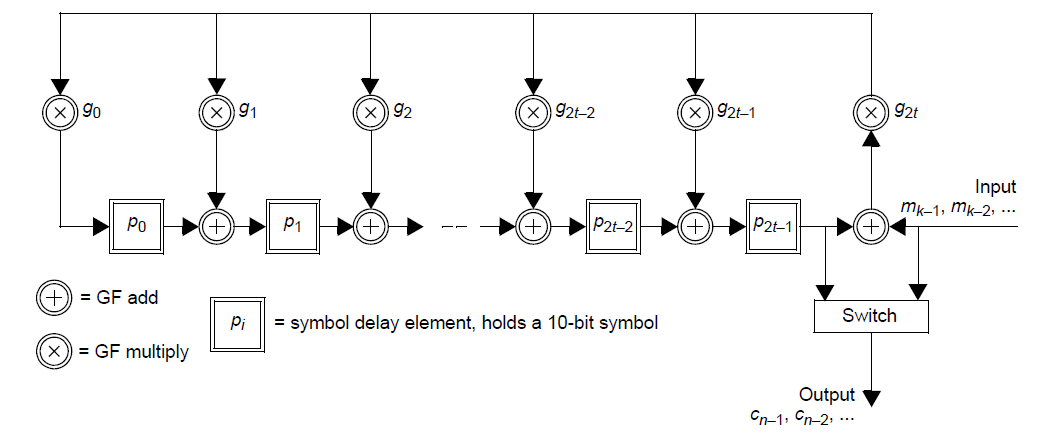
\includegraphics[width=0.95\textwidth,height=0.5\textheight,keepaspectratio]{rs-shift-register.png}
    \caption{Model funkcjonalny kodera RS~\cite[sekcja 91.5.2.7]{Ethernet}}\label{model-funkcjonalny}
\end{figure}
